%%
\section{Methodology}
\label{sec:methodology}

\begin{figure}[!ht]
    \centering
    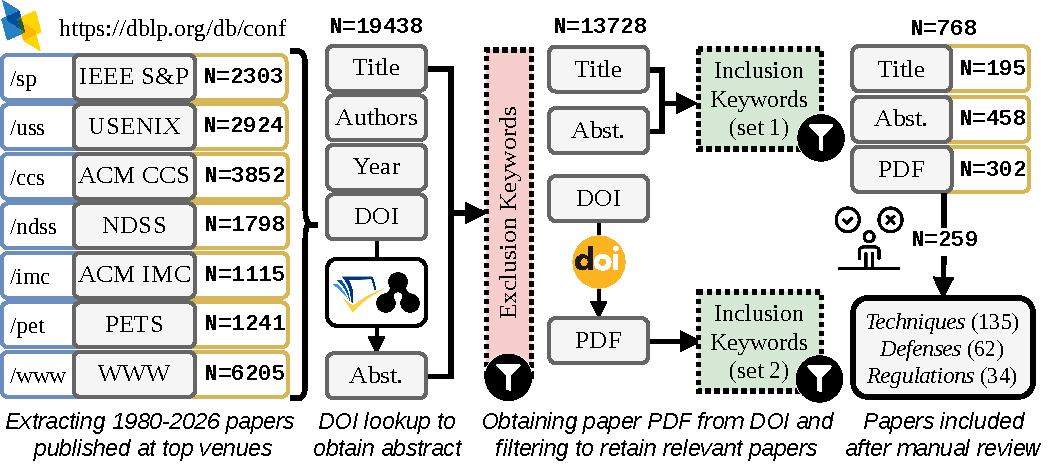
\includegraphics[width=\columnwidth]{figures/methodology.pdf}
    \caption{Overview of our literature search.}
    \label{fig:methodology}
\end{figure}

\subsection{Literature Review}
\label{sec:lit-review}
% 
Online tracking comprises a vast body of literature published over the last few decades---spanning across technical mechanisms, defenses, and regulatory compliance. 
%
To systematize evolution of web tracking, we begin by performing a literature search to identify all papers related to web tracking published at any of the following seven web security and privacy venues---IEEE S\&P, USENIX Security, ACM CCS, NDSS, ACM IMC, PETS, and WWW.

%%
We first identify all papers published at these conferences since their inception (i.e., from 1980 to 2026) using DBLP (\url{https://dblp.org/db/conf}) with conference-specific paths (see~\autoref{fig:methodology})\footnote{For PETS, we use `conf/pet' (2000-2014) \& `journals/popets' (2015+)}. 
%
We obtain a total of 19438 papers along with their metadata (title, authors, year, and DOI). 
%
Since paper abstracts were not always available, we perform a DOI-based query on Semantic Scholar\footnote{\url{https://www.semanticscholar.org/}} and OpenALex\footnote{\url{https://openalex.org/}} to obtain abstracts for each paper. 

%%
Next, to retain papers purely relevant to web tracking techniques, mitigations, and regulations, we use inclusion and exclusion criteria (see~\refappendix{sec:keywords}) based on the presence of certain keywords in the title, abstract, or PDF of these publications. 
%
These keywords were refined over multiple iterations and discussion among the two authors. 
%
First, exclusion keywords remove potential papers that could be incorrectly retained under web tracking. 
%
Second, two sets of inclusion keywords are used to narrow down potential candidates for manual review. 
%
The first set is used to filter publications that are related to web tracking techniques and defenses based on their title and abstract text. 
%
The second set of keywords is used to identify papers discussing privacy regulations and compliance in the context of web tracking in their full text. 
%
We rely on full text search to identify papers that may not primarily be regulation-focused (hence lower probability of a match in title or abstract), but may still discuss regulatory implications of the studied tracking technique or defense in the paper. 
% (an initial query on just title and abstract yielded too few relevant results).

%%
%
We scope this SoK's focus on web tracking in context of desktop and mobile. 
%
To this end, we manually review the filtered 768 candidate papers by discussing among the authors to further exclude publications unrelated to online tracking or those out of scope from our general focus (e.g., tracking in IoT ecosystem, tracking use cases such as online advertising, etc.). 
%
This yielded a final set of 259 research papers related to three web tracking dimensions: measurements and techniques (N=135), defenses (N=62) and regulatory compliance (N=34).


%%
\subsection{Systematization}
% 
To systematize the evolution of web tracking along these three dimensions, we follow Clarke and Braun’s thematic analysis approach~\cite{clarke2013successful} that eliminates the need for inter-rater reliability. 
%
First, one researcher with expertise in web tracking, reviews each included paper to evaluate it based on our systematization criteria listed in Table~\ref{tab:systematization-criteria}. 
%
Next, the evaluator convened with the second expert researcher to deliberate any ambiguities and reach
a consensus on the final evaluation in order to ensure a high quality of analysis as suggested in Clarke and Braun’s approach.
%
The finalized taxonomy for each criteria is listed in Tables~\ref{tab:systematization-criteria}, \ref{tab:??} and \ref{tab:??}.
%
% A total of 40 topical themes were identified (see~\refappendix{sec:thematic-analysis}), with the top 15 (by number of papers) being tracking measurements, tracking in browsers and mobile, browser fingerprinting, regulation compliance, profiling, third-party tracking, cookie consent, cookies, user studies in tracking, ad blocking, JavaScript-based tracking, side-channels, advertising and tracking defenses, and browser extension fingerprinting.
% 
% \subsection{Coding Tracking Techniques and Mitigations Papers}
% \subsection{Coding Regulations and Compliance Papers}
% \subsection{Identifying Advances and Open Problems}
%
We use our domain expertise to structure the SoK around this taxonomy to systematize evolution of tracking techniques, defenses, and regulatory compliance, while identifying gaps and open problems to guide future research. 

%%
\begin{table*}[t]
\centering
\caption{Summary of systematization criteria and taxonomy.}
\label{tab:systematization-criteria}
\renewcommand{\arraystretch}{1.2}
\begin{tabular}{p{0.08cm} p{10.3cm} p{5.9cm}}
\toprule
& \textbf{Criteria and Description} & \textbf{Taxonomy} \\
\midrule

\multirow[c]{7}{*}{\rotatebox[origin=c]{90}{\parbox{2.5cm}{\centering\textbf{Techniques}}}}
 & \textbf{Tracked Artifacts}: What artifacts are used to track users using this tracking technique? & see Table~\ref{tab:} \\
 & \textbf{Tracked State}: What state does this tracking technique maintain to track users? & Stateful, Stateless, Both \\
 & \textbf{Tracking Context}: In what context does this tracking technique function? & Third-party, First-party, Both \\
 & \textbf{Tracker Goals}: What are achievable goals of the tracker employing this tracking? & Same-site, Cross-site, Cross-device \\
 & \textbf{Tracker Capabilities}: What capabilities are required to use this tracking technique? & Inclusion, Execution, Observation, Storage, Sharing \\
 & \textbf{Gaps}: What are potential gap(s) in the evolution of this tracking techniques? & see Section~\ref{sec:} \\
 & \textbf{Open problems}: What are potential future research direction(s) related to this tracking? & see Section~\ref{sec:} \\

\midrule

\multirow[c]{6}{*}{\rotatebox[origin=c]{90}{\parbox{2.2cm}{\centering\textbf{Defenses}}}}
 & \textbf{Tracking technique}: What tracking technique does this tracking defense protect against? & see Table~\ref{tab:} \\
 & \textbf{Defense Artifact}: What tracking artifact(s) does this defense apply protection to? & see Table~\ref{tab:} \\
 & \textbf{Defense Development}: Who developed this tracking defense? & Research-based, Community-based, Industrial \\
 & \textbf{Defense Deployment}: How can or is this defense deployed? & \dNative in-browser, \dExt extension, offline / list-augmentation or auditing tool (\dTool\ );  server-, network-, protocol-, or OS-level (\dServer\ ). \\
 & \textbf{Defense Support}: What is support for this and other related practically deployed defenses? & see Figure~\ref{fig:} for browser-specific support\\
 & \textbf{Gaps}: What are potential gap(s) in the evolution of these tracking defenses? & see Section~\ref{sec:} \\
 & \textbf{Open problems}: What are potential future research direction(s) for defenses? & see Section~\ref{sec:} \\

 \newcommand{\dNative}{\ding{108}} % in-browser
\newcommand{\dExt}{\ding{117}} % extension
\newcommand{\dTool}{\ding{109}} % offline/list tool
\newcommand{\dServer}{\ding{115}} % server/network/protocol/OS
\newcommand{\dNo}{\textemdash}

\midrule

% \multirow[c]{1}{*}{\rotatebox[origin=c]{90}{\parbox{3.8cm}{\centering\textbf{Regulations \&}\\\textbf{Compliance}}}}
%  & & & \\

\bottomrule
\end{tabular}
\end{table*}



\subsection{Approach Limitations}

\noindent We acknowledge the following limitations in our approach.
% with our metho that are inherent from any SoK effort.

\para{Selection Bias.} We scope our SoK to seven of the top security and privacy conferences where web tracking research has been commonly published. Consequently, some publications relevant to web tracking techniques, defenses, and regulations published elsewhere may have been left out from our systematization approach. 
% Mitigations: 
% - broad search further refined automatically on identified exclusion keywords and manual evaluation
% - venues aligned with our expertise and where we have seen most relevant papers in the past to web tracking
% - 

\para{Coding Bias.}
As with any qualitative analysis, our systematization is subject to a degree of subjectivity in how papers are evaluated against the criteria in Table~\ref{tab:systematization-criteria}. We mitigate this following Clarke and Braun's thematic analysis approach~\cite{clarke2013successful}
% , in which two expert researchers collaboratively deliberated ambiguities and refined the taxonomy through consensus
. While this approach reduces inconsistencies, it does not entirely eliminate the possibility that different researchers may arrive at slightly varying interpretations of the taxonomy.
% coding + interpretation
% extracting general and common trends

\para{Regulation Focus on EU and US Contexts.}
% in literature search (keywords)
% but US/EU contexts are the closest to our expertise
% GDRP (+ePD) and CCPA are seen as the precursors and have influenced many other regulations around the world
